\documentclass[a4paper]{article}

% Load the VUB package.
% This has many options, please read the documentation at
% https://gitlab.com/rubdos/texlive-vub
\usepackage{vub}
\usepackage[english]{babel}

% Some highly suggested packages, please read their manuals.
\usepackage{hyperref}
\usepackage{float}
\usepackage{xcolor}
\usepackage{listings}
\usepackage{graphicx}
\usepackage{xparse}
\usepackage{cleveref}
\usepackage[natbib, style=ieee]{biblatex}
\usepackage{csquotes}
\addbibresource{bibliography.bib}
\setlength\parskip{\baselineskip}
\graphicspath{{./images}}
\definecolor{darkred}{rgb}{0.6,0.0,0.0}
\definecolor{darkgreen}{rgb}{0,0.50,0}
\definecolor{lightblue}{rgb}{0.0,0.42,0.91}
\definecolor{orange}{rgb}{0.99,0.48,0.13}
\definecolor{grass}{rgb}{0.11, 0.53, 0.17}
\definecolor{pink}{rgb}{0.97,0.15,0.45}
\definecolor{backcolour}{rgb}{0.95,0.95,0.92}

\newcommand{\secref}[1]{\autoref{#1}.}

\lstdefinestyle{mystyle}{
  basicstyle=\ttfamily,
  backgroundcolor=\color{backcolour},   
  commentstyle=\color{darkgreen}\itshape,
  keywordstyle=\color{blue}\bfseries,
  stringstyle=\color{red},
  showspaces=false,                
    showstringspaces=false,
    showtabs=false,
    breakatwhitespace=false,         
    breaklines=true,                 
    captionpos=b,                    
    keepspaces=true,                 
    numbers=left,                    
    numbersep=5pt,
}

\lstset{language=Python, style=mystyle}
\title{Delivering Actors with Stork}
\pretitle{\flushleft{Bachelor thesis submitted in partial fulfillment of the requirements for the degree of bachelor of science: Computer Science}}
\subtitle{ A distributed computing deployment tool}
\author{Gérard Lichtert}
\date{\today}
\promotors{Promotors: Prof.\ Dr.\ Joeri de Koster and Prof.\ Dr.\ Wolfgang de Meuter. \and Advisor: Mathijs Saey}
\faculty{Sciences and Bio-Engineering sciences}

\begin{document}
\maketitle
\tableofcontents
\newpage
\raggedright{}


\section{Introduction}
In a world of electronics and machines where power consumption is always increasing, optimizing power consumption is becoming increasingly important. While electricity is expensive, the main reason lies in climate change. This is because the majority of our electricity production still comes from non-renewable sources, such as coal, oil, and gas \cite{owid-energy-mix}. These sources produce a lot of CO\textsuperscript{2}, and other greenhouse gases, which are the main contributors to climate change. While there is research being done to optimize energy generation, optimizing power consumption is becoming increasingly important. This means that we as programmers can also play a role in optimizing our programs to consume less energy.

In the world of computing, cloud computing is responsible for 1\% of the worldwide energy consumption \cite{cloudcomputingenergycrisis}. To make use of the cloud, we do not only need electricity to power the devices that provide cloud computing but also electricity to power the network, which also plays a significant role in energy consumption. This is because the network is the backbone of most if not all, communication between devices and applications. The amount of connected devices and applications keeps growing, which leads to higher network usage. Consequently, higher network usage also leads to higher energy consumption, which leads to a higher carbon footprint \cite{RATHEESH}. Higher network usage also requires better infrastructure to handle the increased data volume, which in turn also requires more energy \cite{datavolumeeffects}. To reduce the network load we need to look at the data that is being sent through the network and if we can reduce it.

Data is usually transported through the network for a few reasons. Sometimes it is to send data to a device to update local data, like a chat message that needs to be added to the chat, or a new email that needs to be downloaded. While often compressed, the data is used as-is, and thus cannot be further reduced. Other times, however, data is sent to be processed. This can potentially be optimized by applying the edge-computing principle. This means that (part of) the data that is originally meant for processing is processed locally first, potentially reducing the amount of data that needs to be sent after preprocessing it. Logically, the network load, and consequently the energy consumption, should be reduced. However, for a certain set of devices or applications, it could be optimal to pre-process the complete set of data prior to sending it over the network, while for another set of devices or applications, it could be optimal to send the data directly to the server. Sometimes, however, the optimal configuration could be a combination of the two. We want to be able to experiment with these different configurations. In this work, we focus on the Python programming language, as it is a popular language often used for data science or AI applications running in the cloud. For this purpose, we introduce Stork.

Stork is a distributed computing deployment tool written in Python that makes it possible to deploy distributed systems and try out different configurations regarding these systems. More concretely, it allows us to initialise the deployment of a distributed system, change the configuration of where each part of the distributed system is deployed in a declarative way, and reverse the deployment.

In this thesis, we discuss Stork, how a user can use it and how it is implemented. We start by discussing the background of Stork. Followed by how a user can use Stork. We then discuss how Stork is implemented and finalize the thesis with a conclusion.
\section{Background}
Before we discuss Stork, we discuss the goals that Stork should achieve and how. As mentioned in the introduction, we require a tool that allows us to declare where which data gets processed. This means that we need to be able to deploy parts of our program to different devices. Consequently, this means that our tool needs to work in the context of distributed systems. For this a distributed computing paradigm is required that allows us to deploy our system in a distributed way, as well as change where parts of our programs reside. Next, we discuss the available technologies and libraries in Python and choose the one(s) that best fit our needs.
\subsection{Distributed computing paradigm}
\label{sec:distributedcomputingparadigm}
To start with distributed computing, a suitable distributed computing paradigm that allows our system to be deployed to the cloud without much manual intervention, yet helps us with experimenting different configurations, is required. There are several options, such as:
\begin{itemize}
    \item Message Passing Interface (MPI)\cite{MPI}
    \item Remote Procedure Call (RPC)\cite{RPC}
    \item Shared Memory Model\cite{SMM}
    \item The Actor Model\cite{ActorModel}
\end{itemize}
An Actor is a computational unit that encapsulates its state and behavior, interacting with each other through asynchronous message passing. Each Actor has a mailbox in which it receives these messages and processes them sequentially. The encapsulation property of the Actor Model allows Actors to be very modular, as we can see each Actor as a separate unit that processes part of the data. More concretely, each actor will be responsible for processing a single part of the data. This allows us to easily move parts of the data processing pipeline from one device to another. This is important because we want to be able to change where data gets processed without redefining how it gets processed.

While it is technically possible to achieve modularity in MPI, RPC, and the Shared Memory Model, due to the tight coupling of those models, it is harder to achieve. This is because the state and behavior of the system are not encapsulated in a single entity but rather spread across the entire system. This makes it harder to move parts of the system around. Consequently, we choose the Actor Model as the distributed computing paradigm for Stork.

Using an IoT system as a running example because IoT devices account for 50\% of networked devices\cite{differentnetworkneedsiot}. Say the system exists out of three devices with sensors and a cloud, where the devices feed the sensor data to the cloud. Once the data is in the cloud, it gets processed and stored in a database. It is possible to encapsulate the behavior of each sensor in an Actor and connect this with another Actor responsible for sending the data to a server, where the data gets sent through a series of Actors that are each in turn responsible for processing a single part of the data, just like in Figure \ref{fig:iotActorExample1}.
\begin{figure}[H]
    \centering
    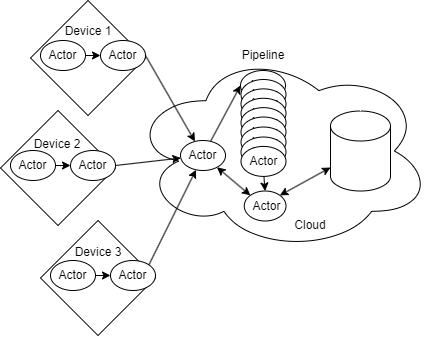
\includegraphics[width=0.6\textwidth]{iotActorExample1.png}
    \caption{An example of an IoT system using the Actor Model}
    \label{fig:iotActorExample1}
\end{figure}
Conceptually, we should be able to spawn some of the Actors that process data from the pipeline to the IoT devices and place them before the Actor that sends the data to the Server. These Actors will pre-process data prior to sending it to the cloud, where the data will go through the rest of the pipeline. The preprocessing Actors that have been moved are coloured blue. Achieving one of the possible configurations without having redefined how the data gets processed.
\begin{figure}[H]
    \centering
    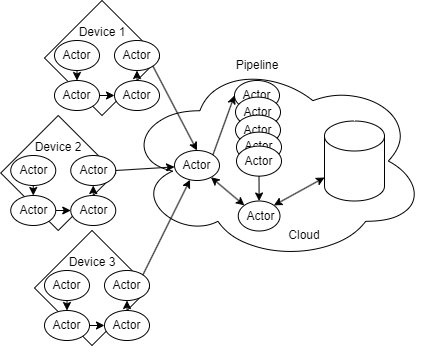
\includegraphics[width=0.6\textwidth]{iotActorsMoved.png}
    \caption{An example of an IoT system where some of the Actors that process data are spawned on the IoT devices instead of the server.}
    \label{fig:iotActorExample2}
\end{figure}
\subsection{Implementing Actors in Python}
When using Stork to deploy distributed systems and try out different configurations, Actors have to be created. However, before we can discuss how to use Stork, we discuss how to implement Actors in Python. In Python, there are two libraries that allow us to implement the Actor Model: Pykka\footnote{https://pykka.readthedocs.io/en/stable/} and Thespian\footnote{https://thespianpy.com/doc/}. Thespian is the only library that supports distribution and distributed communication out of the box, while Pykka does not. Because of this, Thespian is the library of choice for Stork, and consequently, Stork only works with Thespian Actors.

To create an Actor, a class must inherit from a Thespian Actor class. Furthermore, this Actor must at least implement the \lstinline{receiveMessage} method or equivalent, depending on the Actor class that is extended. As mentioned in \secref{sec:distributedcomputingparadigm}, Actors communicate through asynchronous messaging. This means that when the Actor receives a message, it calls the \lstinline{receiveMessage} method. An example of an Actor implementation is given below. This Actor will respond with "Hello World! back" when it receives the message "are you there?".
\begin{lstlisting}[language=Python, caption=Actor example, label=lst:actor]
from thespian.actors import Actor

class HelloWorld(Actor):

    def receiveMessage(self, message, sender):
        if message == "are you there?":
            self.send(sender, "Hello World! back")
\end{lstlisting}
\section{Stork}
Stork is a distributed computing deployment tool, written in Python, that makes it possible to deploy an actor application over a distributed system in several different ways with minimum changes to the code. Stork provides the following features:
\begin{enumerate}
    \item Initializing the distributed system, allowing Actors to be spawned on the declared devices.
    \item De-initializing the distributed system, removing all Actors from the declared devices.
    \item Delivering an Actor class to the devices, allowing the Actor to be spawned on the device. This comes in two variants.
    \item Fetching the references of Actors that have been spawned across the distributed system. This comes in three variants.
    \item sending or broadcasting messages to the spawned Actors.
\end{enumerate}
\subsection{Initializing the distributed system}
When the user of Stork wants to initialize the distributed system, the user has to declare which devices take part of the distributed system. More importantly, Stork needs to know from which of these devices the distributed system should be initialized. This is because Thespian requires a leader device, to which the other devices register themselves to. Stork in turn uses this leader device to keep track of the registered, or remote devices, and spawn Actors on the remote devices and the leader device. It is expected that the user uses this method prior to deploying the user defined Actors. Otherwise the user defined Actors cannot be spawned.
\begin{lstlisting}[language=Python, caption=Initializing the distributed system, label=lst:init]
import Stork

if __name__ == "__main__":
    # First we declare a list of the host names of the devices that have to be part of our distributed system
    devices = ["server@vub.ac.be","device1", "device2", "device3"]
    # Then we call the distributeSystem method, with the leader device being the first host name in the list of devices.
    Stork.distributeSystem(leader=devices[0], convention=devices)
\end{lstlisting}
It is expected that the user calls this method on the leader device, because it is expected that the leader device has access to the other devices.

Alternatively, a user of Stork can instead of declaring the devices in a list, declare them in a dictionary with the keys as the host names and a list of properties as the value. This way the user can declare the capabilities of the devices, which can be used to spawn Actors on the devices that have the requested capabilities.
\begin{lstlisting}[language=Python, caption=Initializing the distributed system with capabilities, label=lst:initcap]
import Stork

if __name__ == "__main__":
    # Just like before we declare our devices, but this time in a dictionary with the host names as keys and the capabilities as values.
    devices = {
        "server@vub.ac.be" : ["server", "database"],
        "device1" : ["sensor"],
        "device2" : ["sensor"],
        "device3" : ["sensor"]
    }
    Stork.distributeSystem(leader=devices.keys()[0], convention=devices)
\end{lstlisting}
Again, it is expected that the user calls this method on the leader device, because it is expected that the leader device has access to the other devices.
\subsection{De-initializing the distributed system}
De-initializing the distributed is the opposite of initializing the distributed system. This is necessary because when the user is done with the distributed system, all processes must be stopped. Since all processes of the Actors are running on the background on the devices declared when calling \lstinline{distributeSystem}, Stork creates a connection with the devices and runs a script to end all Actor related processes. Just like \lstinline{distributeSystem}, it is expected that the user calls this method on the leader device.
\begin{lstlisting}[language=Python, caption=De-initializing the distributed system, label=lst:deinit]
import Stork

if __name__ == "__main__":
    Stork.undistributeSystem()
\end{lstlisting}
\subsection{Delivering an Actor class to the devices}
Now that the methods to initialize and de-initialize the distributed system have been discussed, we can discuss how to distribute the Actors. Whenever the user wants to spawn an Actor on a device, the user can use two different methods to spawn the given Actor class. Stork provides two methods for this: \lstinline|deliverActor| and \lstinline|deliverOrActor|. However, these methods must be called within an Actor. This is because Stork uses the Actor to communicate internally, that an Actor must be spawned on a certain device.

The \lstinline{deliverActor} method takes the Actor calling the method as an argument and a list of capabilities as a second argument. The list of capabilities is used to determine on which devices the Actor should be spawned. Taking a look at the example from listing \ref{lst:initcap}, if we want to spawn an actor on all the devices with the capability \enquote{sensor}, we can use \lstinline{Stork.deliverActor(self, ActorClass, ["sensor"])}. However, if we only want to spawn the Actor on one of the sensors, we can use \lstinline{Stork.deliverActor(self, ActorClass, ["device1"])}, or \lstinline{Stork.deliverActor(self, ActorClass, ["sensor", "device1"])}. Regardless, \lstinline{deliverActor} will spawn the Actor on all devices that have the all requested capabilities.
\vfill
\begin{lstlisting}[language=Python, caption=Delivering an Actor, label=lst:deliverActor]
import Stork
from thespian.actors import Actor

class Pong(Actor):

    def receiveMessage(self, message, sender):
        self.send(sender, "pong")

class Ping(Actor):

    def receiveMessage(self, message, sender):
        if message == "spawn":
            Stork.deliverActor(self, Pong, ["sensor"])
\end{lstlisting}

Now that Stork spawned Actors on all the devices that have the \enquote{sensor} capability, how does a user of Stork interact with them? As mentioned in \secref{sec:distributedcomputingparadigm}, Actors communicate through asynchronous messaging. In Thespian and therefore Stork, this means that when a message is sent from an Actor to another Actor, it will never receive a return value. \lstinline|deliverActor| and \lstinline|deliverOrActor| are no exceptions to this rule, since they work in a similar manner. However, when an Actor sends a message to another Actor it can send a message back. Consequently, the user of Stork needs to extend the \lstinline|receiveMessage| method to handle the message that Stork sends to the Actor calling the delivery methods. This message contains the references to the Actors that have been spawned, as well as the hostname of the device where the Actors were spawned. Once the Ping Actor has the references of the Pong Actors it can interact with the Pong Actors in a similar manner as it would with other thespian Actors.

For this purpose, Stork also provides a class to easily encapsulate the message that is sent to the Actor that called the delivery methods. This class is called \lstinline|DeliveredActors|. The \lstinline|DeliveredActors| class understands the following methods:
\begin{enumerate}
    \item \lstinline{unpackActors()}: This method returns a dictionary with the host names of the devices as keys and another dictionary as value. The dictionary as value has the spawned Actor class as keys and the reference as value. This way we can address the Actor not only by the device that it is on but also by the class. Using the example from listing \ref{lst:deliverActor}, the dictionary would look like this:
          \begin{lstlisting}[language=Python]
{
    "device1": { Pong: reference_to_Pong },
    "device2": { Pong: reference_to_Pong },
    "device3": { Pong: reference_to_Pong }
}
    \end{lstlisting}
    \item \lstinline{emit(self: Actor, host: str, Actorclass: Actor, message: Any)}: This method sends a message to the Actor that was spawned on the device with the given host name.
    \item \lstinline{broadcastHost(self: Actor, host: str, message: Any)}: This method sends a message to all the Actors that were spawned on the device with the given host name.
    \item \lstinline{broadcast(self: Actor, message: Any)}: This method sends a message to all the Actors that were spawned.
\end{enumerate}
As with the \lstinline|deliverActor| method, the \lstinline|DeliveredActors| class must be used within an Actor. This is because the \lstinline|DeliveredActors| class uses the Actor to send messages to other Actors.

\begin{lstlisting}[language=Python, caption=Receiving the references of the spawned Actors and broadcasting "ping", label=lst:receive]
import Stork
from thespian.actors import Actor

class Pong(Actor):

    def receiveMessage(self, message, sender):
        self.send(sender, "pong")

class Ping(Actor):

    def receiveMessage(self, message, sender):
        if message == "spawn":
            Stork.deliverActor(self, Pong, ["sensor"])
        elif isinstance(message, Stork.DeliveredActors):
            message.broadcast("ping")
        
\end{lstlisting}

The \lstinline{deliverOrActor} method works in a similar way as the \lstinline{deliverActor} method. The difference lies in the way the capabilities are checked. With \lstinline|deliverActor| the device must have all specified capabilities. With \lstinline|deliverOrActor| it suffices that the device has one of the required capabilities. Other than that it works in the same way as \lstinline|deliverActor|. It will also send a message to the Actor that called the method, containing the references to the spawned Actors in the \lstinline|DeliveredActors| class.

Sometimes however, an Actor is already created and a reference of said Actor is needed to communicate with it. Stork provides three methods for this. The first one only gets the address of a single Actor class of a specific device. This can be done with \lstinline|Stork.getActorAddress| which expects the Actor calling it as first argument, the host name of the device we want to get the reference of, and the class of the Actor that we want to get a reference of. Essentially the same as the \lstinline|DeliveredActors.emit| method but without the message parameter.

The second method is \lstinline|Stork.getActorClassAddresses| which works similarly to \lstinline|DeliveredActors.broadcastHost|. However instead of the hostname it expects a class. More concretely, it expects the Actor calling it as the first argument and the Actor class of which we want to get addresses as the second argument. \lstinline|Stork.getActorClassAddresses| gets all the addresses of the Actors of a specific class.

Thirdly and lastly there is \lstinline|Stork.getActorHostAddresses| which works similarly to \lstinline|DeliveredActors.broadcastHost|, but without the message parameter. It expects the Actor calling it as the first argument and the host name of the device of which we want to get the references of the Actors as the second argument. \lstinline|Stork.getActorHostAddresses| gets all the addresses of the Actors on a specific device.

Just like in \ref{lst:deliverActor} the response has to be handled in the \lstinline{receiveMessage} method. For these methods Stork provides another class, to differentiate it from the \lstinline|DeliveredActors| class. This class is called \lstinline|ActorAddresses| and has the same methods as \lstinline|DeliveredActors|.
\section{Implementing Stork}
Now that we have discussed the features that Stork provides, we can discuss how it is implemented. As previously mentioned, Stork is built on Thespian, a Python Actor library. This means that most features that Stork provides are built on Thespian. But, perhaps it is worth discussing why Thespian, and not another Python Actor library, as there is another one called Pykka.

Pykka is a Python implementation of the Actor Model. It introduces some simple rules to control the sharing of state and cooperation between execution units, which makes it easier to build concurrent applications\footnote{https://pykka.readthedocs.io/en/stable/}. However, Pykka does not support distributed communication out of the box, like Thespian does. This is important since we we want to build a distributed system. Consequently, we choose Thespian over Pykka.

Before discussing the implementation of Stork there are a few things that must be discussed about Thespian. When creating Actors it must be done within an ActorSystem. Meaning that on every device, on which we want to create an Actor, an ActorSystem must be present. This is because the ActorSystem manages the Actors and their communication. Consequently this means that an active ActorSystem is required on each device before we can create an Actor. This can be done by running a small script that creates an ActorSystem, nothing more, since the ActorSystem will be running in the background. This means we need to SSH to all devices and run the script on each device. For a small amount of devices this probably will not be an issue if it has to be done once or twice. However, when the distributed system is large, or the deployment is repetitive, it will be very taxing to the deployer, since it is a lot of repetitive manual work.

\subsection{Automating the deployment of ActorSystems}
For this we require to implement a program that automatically SSH's to the all devices of the distributed system and runs the script to create an ActorSystem. However, the order is important. Thespian calls these distributed systems \enquote{a convention}. Each convention must have a convention leader, to which the other ActorSystems register themselves to.
To automate this, we need a library or technology that serves as infrastructure as code (IaC). The options are:
\begin{enumerate}
    \item Ansible
    \item Fabric
    \item Chef
    \item Puppet
    \item Terraform
\end{enumerate}
Most of these IaC tools are quite heavyweight and would require us to learn another language. Fabric however is a Python library that allows the user to create SSH connections and run commands on remote devices. This is perfect for our use case, as we are using Python to create the script that creates the ActorSystem, and thus allows us to stay in the same language. Consequently, we can use Fabric to automate the creation of the ActorSystems on the devices.

There is still one issue though, when using Fabric to create a SSH connection and running a command, it expects that the process returns. It does so because it expects the command to be a foreground process. However, when creating an ActorSystem, as this starts a background process, it never returns. This is circumvented by using \enquote{tmux} before executing the program to start the ActorSystem. This ensures that the process is running in the background and the command returns. This is also how the \lstinline|Stork.distributeSystem| works, as it uses Fabric to create the ActorSystems on the devices. The \lstinline|Stork.undistributeSystem| method works in a similar way, as it uses Fabric to stop the ActorSystems on the devices. This is done by running a script that stops the ActorSystem on the devices. This script is also run in a \enquote{tmux} session, to ensure that the command returns. Essentially, both Stork methods call methods implemented for Fabric that create a SSH connection to the devices and run a command, that runs the initialization or de-initialization script. Hence the importance that this is done from the leader device.

\subsection{Creating and delivering Actors}
The \lstinline|Stork.deliverActor| and \lstinline|Stork.deliverOrActor| methods work in a different manner, though they do make use of the ActorSystems that have been created by the \lstinline|Stork.distributeSystem| method. In Thespian there are two ways to create Actors. One through the ActorSystem and one through an Actor, meaning that Actors can create other Actors.
This begs the question of how we can create Actors on remote devices? More specifically from the leader device, since we do not want to have to SSH to the remote devices to create Actors there. While Thespian does support a mechanism to restrict the creation of certain Actor classes to certain devices, there is no way to guarantee that the Actor is created on multiple different devices. This is because Thespian will always create an Actor on the first ActorSystem it can. Consequently, most of the times it will spawn the Actor on the same ActorSystem.
Creating a remote Actor from the local ActorSystem is no good either, as it will either create it locally or, when using the Thespian mechanism, it will throw an error that it cannot create that Actor. This is because the mechanism only works when creating Actors from Actor, however, as mentioned before it does not work when the user wants to create an instance of an Actor on multiple devices.

To work around this, we implement an administrative Actor that has to run on the leader device. As there is only one instance of the administrative Actor, we can use Thespians restriction mechanism to our advantage. This means that we can restrict the creation of the administrative Actor to the leader device. When running the scripts to initialize the ActorSystems on all devices, the script now also creates a reference to this administrative Actor. Meaning that all remote ActorSystems are now able to communicate with an administrative Actor on the leader device. However, this still does not guarantee that the references are all pointing to the same administrative Actor. Meaning that if two remote ActorSystem ask the administrative Actor for a reference to a certain Actor, they will likely not get the same response, because they will not be asking the same Actor. This is an issue. To work around this, Thespian provides another feature called the \enquote{global Actor}, which essentially gives the Actor a name, and thus now all remote ActorSystems referencing the administrative Actor will be referencing the same Actor. To prevent users of Stork having a name clash with the administrative Actor, the name is a generated hash.

Now that we have an administrative Actor that can be referenced by all remote ActorSystems, we can use this Actor to fetch addresses as well as create Actors on the leader device. However, We cannot yet create Actors on remote ActorSystems. To achieve this, we create another administrative Actor, called a manager Actor, the manager Actor will be created on all remote ActorSystems. The only thing that the manager Actor does is, register itself with the administrative Actor, create Actors on the device it resides in, followed by returning the reference of the Actors it created to an aggregator Actor. The aggregator Actor is created by the administrative Actor to collect the references of the created Actors, as per the aggregator pattern \cite{aggregatorpattern}. The manager Actor registers itself to the administrative Actor by sending its reference to the administrative Actor, as well as the hostname of the device it resides in. This way the administrative Actor can ask the manager Actor to create an Actor on the device it resides in. The manager Actor then creates the Actor and forwards the reference to the aggregator Actor. When all the references are collected by the aggregator Actor, it sends the result back to the administrative Actor as well as to the Actor that requested the creation of the Actors. This way other Actors can ask the administrative Actor for the addresses of the Actors that were created on the remote devices, and the Actor that originally requested the creation of the Actors has the reference of the Actors that were created on the remote devices. As an example we can use the Ping and Pong Actor classes from listing \ref{lst:receive}

When a user wants to create a Pong actor on the device with the capability \enquote{sensor} from the Ping Actor which is on a remote device. The Ping Actor sends a request to the administrative Actor on the leader device to create a Pong Actor on all the devices with the \enquote{sensor} capability.
\begin{figure}[H]
    \centering
    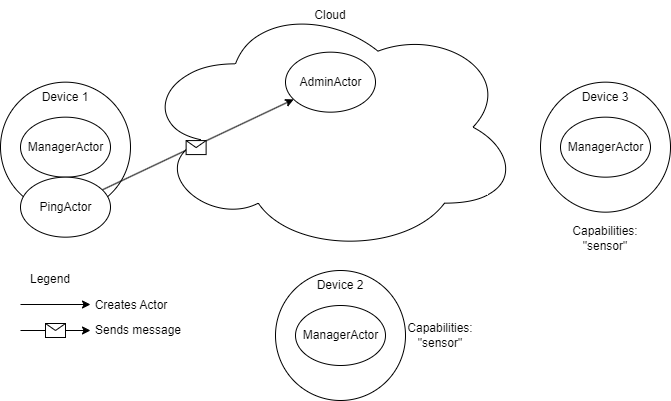
\includegraphics[scale=0.5]{createActor1.png}
    \caption{Ping sends a request to spawn Pong Actors on all devices with the \enquote{sensor} capability}
    \label{fig:createActor1}
\end{figure}
When the administrative Actor processes this request, it collects the references of the registered manager Actors that that are on remote devices with the requested capability. It counts the amount of manager Actors that it should create the Pong Actor and creates an aggregator Actor. The administrative Actor sends to the aggregator Actor the reference of the Ping Actor, that requested the creation of the Pong Actors, as well as the expected amount of results. Furthermore the administrative Actor forwards the creation request to the Manager Actors with the reference of the Aggregator Actor.
\begin{figure}[H]
    \centering
    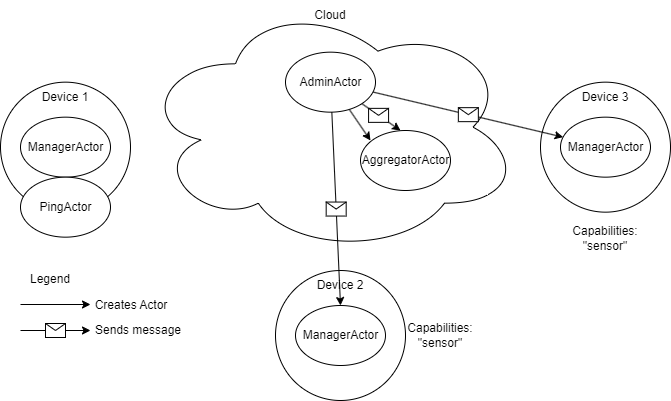
\includegraphics[scale=0.5]{createActor2.png}
    \caption{The creation request is forwarded and an aggregator Actor is created to collect the references of the created Actors}
    \label{fig:createActor2}
\end{figure}
Upon receiving the creation request from the administrative Actor, the Manager Actor creates the Pong Actor and sends the reference of the Pong Actor to the aggregator Actor.
\begin{figure}[H]
    \centering
    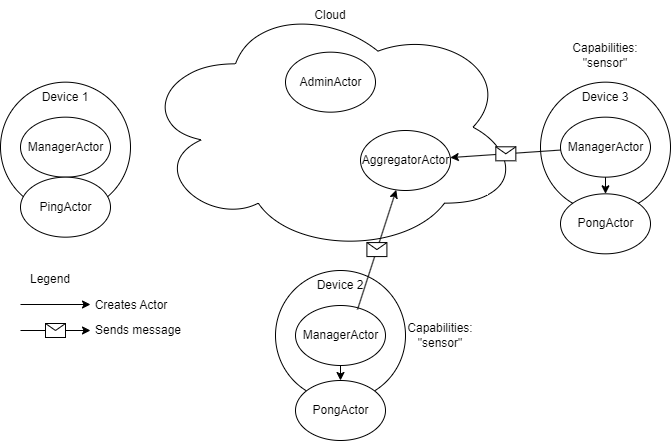
\includegraphics[scale=0.5]{createActor3.png}
    \caption{The Manager Actor creates the Pong Actor and sends the reference to the aggregator Actor}
    \label{fig:createActor3}
\end{figure}
When the aggregator collected all the expected results, it sends the collected references to both the Ping Actor as well as the administrative Actor. The administrative Actor will update its collection of Actor references while the Ping actor will only get the created references.
\begin{figure}[H]
    \centering
    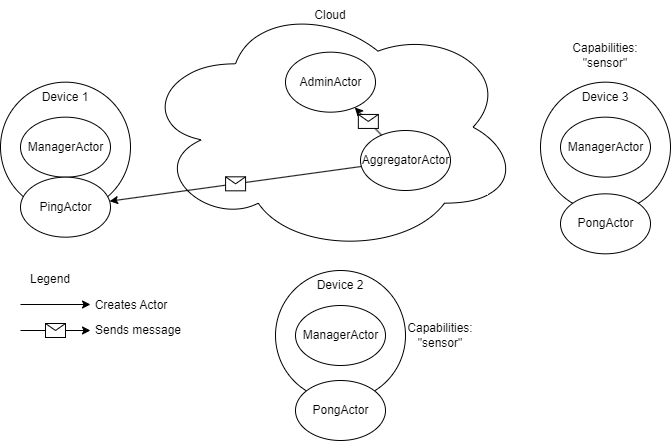
\includegraphics[scale=0.5]{createActor4.png}
    \caption{The aggregator Actor sends the collected references to the Ping Actor and the administrative Actor}
    \label{fig:createActor4}
\end{figure}
This concludes the creation of the Pong Actors on the remote devices, however in the example from listing \ref{lst:receive} the Ping Actor also sends a message to the Pong Actors. While this can be done with looping over the references and sending the message, it helps to have a method that can send a message to all the created Actors, or a subset of the created Actors. For this purpose the methods from the \lstinline|DeliveredActors| are implemented. Schematically it goes as follows:
\begin{figure}[H]
    \centering
    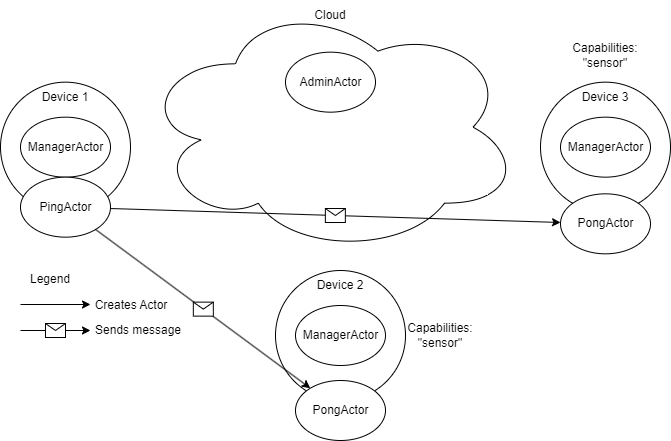
\includegraphics[scale=0.5]{createActor5.png}
    \caption{Ping broadcasts "ping" to all the created Pong Actors}
    \label{fig:createActor5}
\end{figure}
\begin{figure}[H]
    \centering
    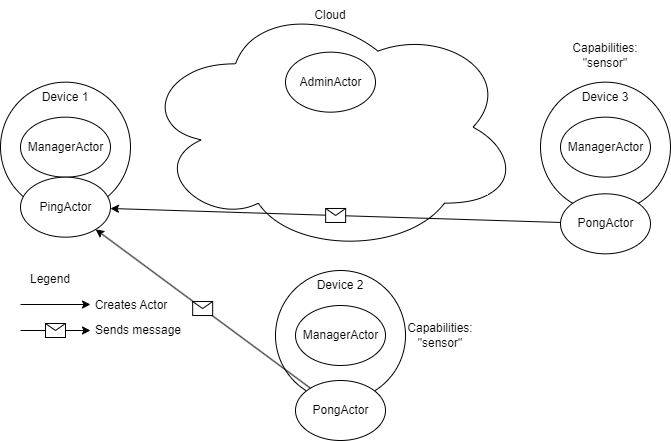
\includegraphics[scale=0.5]{createActor6.png}
    \caption{The Pong Actors receive the message and send "pong" back to the Ping Actor}
    \label{fig:createActor6}
\end{figure}
\subsection{Getting Actor references}
The \lstinline|Stork.getActorAddress|, \lstinline|Stork.getActorClassAddresses| and \lstinline|Stork.getActorHostAddresses| methods work in a similar manner. However the requests do not go further than the administrative Actor, as depicted in figure \ref{fig:createActor1}. The administrative Actor will collect the results from its collection and return the results to the Actor that requested the references. Like with the \lstinline{DeliveredActors} class, it could prove to be useful if we can interact with the Actors directly, instead of the user having to implement a method themselves. This is why the \lstinline{ActorAddresses} class has the same methods as the \lstinline{DeliveredActors} class.
\section{Conclusion}
At the beginning of this bachelor thesis, we wanted to be able to try out different configurations of distributed systems, without much manual intervention. We wanted to do this to see which configuration was the most energy efficient. To achieve this, we introduced Stork, a distributed computing deployment tool, written in Python that makes it possible to deploy distributed systems and removes the overhead of having to SSH to each device to initialize the distributed system manually. It also provides features to create Actors on remote devices, which is necessary to try out a configuration of the distributed system. To test out another configuration of the distributed system, or more concretely moving Actors around. It suffices for the user to change the flow of data, call the \lstinline|Stork.undistributeSystem| method, change the configuration of the capabilities that each device has, and call \lstinline|Stork.distributeSystem| again, before creating the Actors.

Essentially it boils down to changing the flow of data and changing some strings in a dictionary. This is a lot less work than having to SSH to each device manually, start an ActorSystem on each device and then return to the leader device. Especially when the user will still be required to create the Actors on the leader device, SSH to the remote devices again to create the Actors there and then return to the leader device to try out a single configuration. Depending on the amount of devices, configurations and the amount of times the user wants to try out a configuration, this can be very time consuming and not to mention energy inefficient, especially when a tool like Stork exists.
\printbibliography
\end{document}